\chapter{Continuous contrast variation applied to relevant bio-materials}
\label{chap:bio_applications}

The application of nanoparticles (NPs) in medicine opened the continuously growing field of nanomedicine. The first approved nano-drug was Doxil® (Caelyx® in Europe), a PEGylated liposomal formulation of doxorubicin, which was followed by a few other products. Nowadays there are approximately 250 nanomedicine products that are either approved by the relevant health agencies or are under clinical trials. On the other hand, there is a translational gap between the experimental work devoted to the development of new nano-drug candidates and the clinical realization of their use, which is also reflected in the high number of studies dealing with nanomedicine and the number of approved products on the market. As highlighted in a recent review by Khorasani et al. one of the main reasons for this translational gap is that the current characterization techniques possess limitations and there is a need for standardization on this field.

Among many relevant physicochemical properties of nano-drugs, one of the most important to be accurately determined is the size of the nanocarriers, which directly relates to the in vivo biodistribution of the drug. The ultimate goal in this regard is to reach a ‘traceable size determination’ of the nanomaterial, which means that the measurand can be related to the SI unit ‘meter’ through an unbroken chain of comparisons with known uncertainties. 

The most widely used technique for size determination in the field of nanomedicine is dynamic light scattering (DLS), which measures the hydrodynamic diameter of the nanoparticles (NPs). DLS is well-established and has indisputable advantages in the size characterization of the NPs, e.g. easy-to-use instrumentations, fast and low-cost operation, but it is not capable of a traceable size determination as there is no general relationship between the hydrodynamic diameter and the physical size of the NPs. 

Transmission electron microscopy (TEM) is also frequently used for sizing of NPs and proved to be an appropriate technique for solid nanoparticles, whilst its employment in soft matter NPs (e.g. liposomes, micelles and polymeric nanoparticles) is questionable due to the possible distortion of the particles during the drying process.  Although cryo-TEM could overcome this limitation, the statistical accuracy of this non-ensemble method is usually not sufficient.
 
This paper describes a novel approach in small-angle X-ray scattering (SAXS) to assess the size of a complex liposomal drug. SAXS is based on the elastic scattering of X-ray photons by the sample’s electrons at low angles. In contrast to protein crystallography or wide-angle X-ray scattering (WAXS), where the material is characterized at the atomic length scale by collecting the scattering pattern at wide angles, SAXS can provide structural information on nanomaterials in the 1 nm to 300 nm size range. Moreover, SAXS is capable of traceable size determination for sufficiently monodisperse nanoparticles.

In order to perform accurate SAXS measurements, monochromatic, highly collimated X-ray radiation is required with a wavelength below 1 nm, which is perfectly suited to probe materials on the nanoscale. The forward scattered radiation is recorded at small angles (typically up to 3 degrees) with a large area pixel detector placed at a variable distance from the sample (usually from 1 m to 5 m). The one-dimensional scattering intensity curve as a function of the scattering angle is obtained by radial averaging of the two dimensional scattering pattern. In SAXS, the structural properties of the nanomaterials are obtained either from the integral scattering parameters (e.g. Guinier radius, isoscattering point) or by fitting to the scattering curves a known analytical model related to the measured object.
The use of SAXS in liposome research is widespread. For instance, it has been applied to characterize the lamellarity, bilayer thickness, area per lipid ratio and the thickness of the PEG-layer of different liposomal samples, also to describe the influence of extrusion on the average number of bilayers and to determine the electron density profile of liposomes and biological vesicles.

Despite SAXS being a usual method of choice for the accurate size determination of nanomaterials, the interpretation of the scattering curves, i.e. the uniqueness of the solution of the model fitting, is frequently intricate for complex samples. Liposomal drugs belong to this class, as the inner structure of the phospholipid bilayer and the incorporated drug also contribute to the scattering intensity. Presumably this difficulty explains the absence of SAXS studies determining the overall size of liposomal drugs. In general, SAXS characterization of NPs with a broad size distribution, a heterogeneous composition or with a complicated inner structure require either a priori knowledge about the morphology of the sample or the measurement of complementary scattering curves obtained under different experimental conditions. 

Solvent contrast variation in SAXS belongs to the latter approach as it is based on the variation of the scattering curves caused by the addition of a suitable contrast agent to the suspending medium. Recording the scattering data as a function of the adjusted contrast enables the derivation of the mean outer size of the particles irrespective of their inner structure and delivers more detailed information about the NPs composition as compared to single-contrast measurements. In this paper we present an accurate description of a commercially available liposomal doxorubicin sample, which is already in clinical use, with a novel approach to SAXS contrast variation. By creating a solvent density gradient within a capillary, a continuous range of contrasts becomes available, which enables the detailed study of the mean size of the drug carrier, its structural behaviour under different solvents and the nature of the osmotic shrinkage of the liposomal nanocarrier.

\section{Materials and methods}
The solvent density gradient was prepared in vacuum-proof borosilicate glass capillaries from Hilgenberg (Malsfeld, Germany) with a rectangular cross section of (4.2 $\pm$ 0.2) x (1.25 $\pm$ 0.05) mm$^2$, a length of (80 $\pm$ 0.5) mm and a wall thickness of ca. 120 $\eta$m. The bottom end of the capillary was closed by welding and the lower section, up to a height of ca. 1 cm, was filled with Galden R PFPE SV90 from Solvay Plastics (Brussels, Belgium). This fluid has an exceptionally high density of 1.69 g/cm$^3$, low viscosity and is immiscible with aqueous solutions. Consequently, a uniform interface with the particle suspension is formed at the bottom which serves as reference for the transmittance measurements. The suspending medium contrast variation study was performed with the iso-osmolar contrast agent Optiprep® (an aqueous solution of iodixanol), which has an osmolality of 290 to 310 mOsm kg$^{-1}$. The suspending medium density gradient was achieved by bringing together two mixtures of different densities: For the bottom of the capillary, a high density mixture of Caelyx R with Optiprep TM was prepared with an Optiprep TM mass fraction of 35 $\%$ and a corresponding solvent electron density of 365.2 nm$^{-3}$, whilst on the top side of the capillary a low density preparation of Caelyx R  using phosphate buffered saline solution (pH 7.4) with the same volume fraction of Caelyx R was introduced, with a solvent electron density of 341.9 nm$^{-3}$. By employing Optiprep TM as a contrast agent, the osmolality is constant along the capillary. 

In order to study the effects of the suspending medium osmolality in the liposomal drug carrier, another capillary with a density gradient was created by introducing a dense aqueous sucrose solution with 37.8 $\%$ sucrose mass fraction (Sigma-Aldrich, Missouri, USA) at the bottom of the capillary (which corresponds to an electron density of 381.1 nm-3 and a solvent osmolality of 1775.6 mOsm kg$^{-1}$), whereas a lighter solution was produced without sucrose by adding pure water to get the same Caelyx R concentration. Considering the sucrose mass fraction of the Caelyx® buffer to be 10$\%$, this latter preparation has an electron density of 339.4 nm$^{-3}$ and an osmolality of 151.1 mOsm kg$^{-1}$. For the wide-angle X-ray scattering measurements, a density gradient capillary was prepared using a denser aqueous solution with a sucrose mass fraction of 34$\%$ and a lighter one with 6$\%$.

The scattering experiments were performed at the four-crystal monochromator beamline of PTB supplemented by the SAXS setup of Helmholtz-Zentrum Berlin at the synchrotron radiation facility BESSY II (Helmholtz-Zentrum Berlin, Germany). After the gradient was created within the capillary, the sample was moved in steps of 0.5 mm along the central vertical axis of the capillary and a scattering pattern was measured at each position with an exposure time of 60 seconds. At these positions, the solution transmittances were also measured and the suspending medium electron density calibrated as described elsewhere. The momentum transfer q of the scattering curves was calculated from the expression q = E / hc where theta is half of the scattering angle, E = (8000.0 $\pm$ 0.8) eV is the energy of the incoming X-ray radiation, h is the Planck constant and c is the speed of light. The scattered X-ray photons were collected with a vacuum-compatible Pilatus 1M hybrid-pixel detector (Dectris Ltd, Baden,Switzerland) with a pixel size of d = (172.1 $\pm$ 0.2) $\eta$m at a distance L = (4575 $\pm$ 1) mm from the capillaries. The obtained scattering curve was normalized to the exposure time, the measured suspension transmittance and the incident photon flux, measured by means of a calibrated transparent silicon diode. A wide-angle configuration was employed to observe the diffraction peak of the fiber-like doxorubicin precipitate encapsulated in the liposomes. At this configuration, the sample-to-detector distance was reduced to L = (569 $\pm$ 1) mm and as a result the available q-range was extended until 5.55 nm$^{-1}$ X-ray transmission measurements at the aqueous sucrose gradient were performed at a lower incident photon energy E = 5500 eV to increase the transmittance differences for the less absorbing sucrose solution by a factor of 5.

\subsection{Caelyx: PEGylated liposomal doxorubicin}
The PEGylated liposomal formulation of doxorubicin, Caelyx R (SP Europe, Brussels, Belgium), was purchased from Hungaropharma Ltd. Caelyx R (or Doxil R in US) consist of liposomes formed by fully hydrogenated soy phosphatydilcholine (HSPC), cholesterol, and DSPE-PEG2000 (N-(carbonyl-methoxypolyethylene glycol 2000)-1,2-distearoyl-sn-glycero-3-phosphoethanolamine). The latter results a steric barrier at the liposomal surface due to the PEG 2000 residues. Doxorubicin is encapsulated in Caelyx R via an active loading procedure, which results a crystal-like doxorubicin precipitate inside the liposomes, as depicted schematically in figure 0. 

\begin{figure}
	\centering
		\subfloat[Cryo-TEM]{\resizebox{0.4\linewidth}{!}{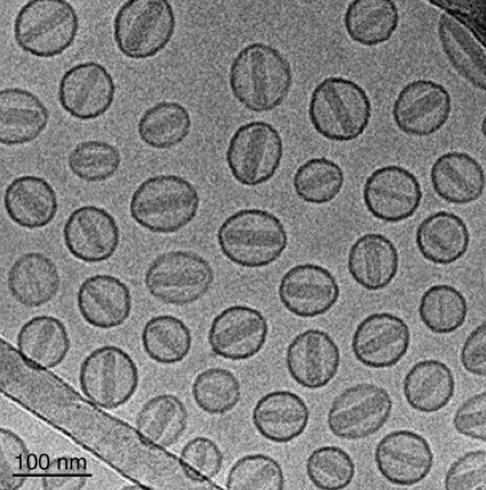
\includegraphics{Figures/CaelyxCryoTEM.png}}\label{fig:CaelyxCryoTEM}}
		\subfloat[Scheme]{\def\svgwidth{0.7\linewidth}{\input{Figures/CaelyxScheme.pdf_tex}}\label{fig:CaelyxScheme}}
		\caption{ Schematic representation of the PEGylated liposomal doxorubicin morphology.}
\end{figure}

\begin{figure}
	\centering
		% GNUPLOT: LaTeX picture with Postscript
\begingroup
  \makeatletter
  \providecommand\color[2][]{%
    \GenericError{(gnuplot) \space\space\space\@spaces}{%
      Package color not loaded in conjunction with
      terminal option `colourtext'%
    }{See the gnuplot documentation for explanation.%
    }{Either use 'blacktext' in gnuplot or load the package
      color.sty in LaTeX.}%
    \renewcommand\color[2][]{}%
  }%
  \providecommand\includegraphics[2][]{%
    \GenericError{(gnuplot) \space\space\space\@spaces}{%
      Package graphicx or graphics not loaded%
    }{See the gnuplot documentation for explanation.%
    }{The gnuplot epslatex terminal needs graphicx.sty or graphics.sty.}%
    \renewcommand\includegraphics[2][]{}%
  }%
  \providecommand\rotatebox[2]{#2}%
  \@ifundefined{ifGPcolor}{%
    \newif\ifGPcolor
    \GPcolortrue
  }{}%
  \@ifundefined{ifGPblacktext}{%
    \newif\ifGPblacktext
    \GPblacktextfalse
  }{}%
  % define a \g@addto@macro without @ in the name:
  \let\gplgaddtomacro\g@addto@macro
  % define empty templates for all commands taking text:
  \gdef\gplbacktext{}%
  \gdef\gplfronttext{}%
  \makeatother
  \ifGPblacktext
    % no textcolor at all
    \def\colorrgb#1{}%
    \def\colorgray#1{}%
  \else
    % gray or color?
    \ifGPcolor
      \def\colorrgb#1{\color[rgb]{#1}}%
      \def\colorgray#1{\color[gray]{#1}}%
      \expandafter\def\csname LTw\endcsname{\color{white}}%
      \expandafter\def\csname LTb\endcsname{\color{black}}%
      \expandafter\def\csname LTa\endcsname{\color{black}}%
      \expandafter\def\csname LT0\endcsname{\color[rgb]{1,0,0}}%
      \expandafter\def\csname LT1\endcsname{\color[rgb]{0,1,0}}%
      \expandafter\def\csname LT2\endcsname{\color[rgb]{0,0,1}}%
      \expandafter\def\csname LT3\endcsname{\color[rgb]{1,0,1}}%
      \expandafter\def\csname LT4\endcsname{\color[rgb]{0,1,1}}%
      \expandafter\def\csname LT5\endcsname{\color[rgb]{1,1,0}}%
      \expandafter\def\csname LT6\endcsname{\color[rgb]{0,0,0}}%
      \expandafter\def\csname LT7\endcsname{\color[rgb]{1,0.3,0}}%
      \expandafter\def\csname LT8\endcsname{\color[rgb]{0.5,0.5,0.5}}%
    \else
      % gray
      \def\colorrgb#1{\color{black}}%
      \def\colorgray#1{\color[gray]{#1}}%
      \expandafter\def\csname LTw\endcsname{\color{white}}%
      \expandafter\def\csname LTb\endcsname{\color{black}}%
      \expandafter\def\csname LTa\endcsname{\color{black}}%
      \expandafter\def\csname LT0\endcsname{\color{black}}%
      \expandafter\def\csname LT1\endcsname{\color{black}}%
      \expandafter\def\csname LT2\endcsname{\color{black}}%
      \expandafter\def\csname LT3\endcsname{\color{black}}%
      \expandafter\def\csname LT4\endcsname{\color{black}}%
      \expandafter\def\csname LT5\endcsname{\color{black}}%
      \expandafter\def\csname LT6\endcsname{\color{black}}%
      \expandafter\def\csname LT7\endcsname{\color{black}}%
      \expandafter\def\csname LT8\endcsname{\color{black}}%
    \fi
  \fi
  \setlength{\unitlength}{0.0500bp}%
  \begin{picture}(5668.00,4534.00)%
    \gplgaddtomacro\gplbacktext{%
      \csname LTb\endcsname%
      \put(946,1162){\makebox(0,0)[r]{\strut{} 1}}%
      \put(946,2313){\makebox(0,0)[r]{\strut{} 10}}%
      \put(946,3464){\makebox(0,0)[r]{\strut{} 100}}%
      \put(2391,484){\makebox(0,0){\strut{} 0.1}}%
      \put(5271,484){\makebox(0,0){\strut{} 1}}%
      \put(176,2486){\rotatebox{-270}{\makebox(0,0){\strut{}Scattering Intensity / a.u.}}}%
      \put(3174,154){\makebox(0,0){\strut{}$q$ / nm$^{-1}$}}%
    }%
    \gplgaddtomacro\gplfronttext{%
      \csname LTb\endcsname%
      \put(4284,4096){\makebox(0,0)[r]{\strut{}Caelyx in buffer}}%
      \csname LTb\endcsname%
      \put(4284,3876){\makebox(0,0)[r]{\strut{}Caelyx in 9.1$\%$ iodixanol}}%
      \csname LTb\endcsname%
      \put(4284,3656){\makebox(0,0)[r]{\strut{}SSL in buffer}}%
      \csname LTb\endcsname%
      \put(4284,3436){\makebox(0,0)[r]{\strut{}Vesicle fit}}%
    }%
    \gplbacktext
    \put(0,0){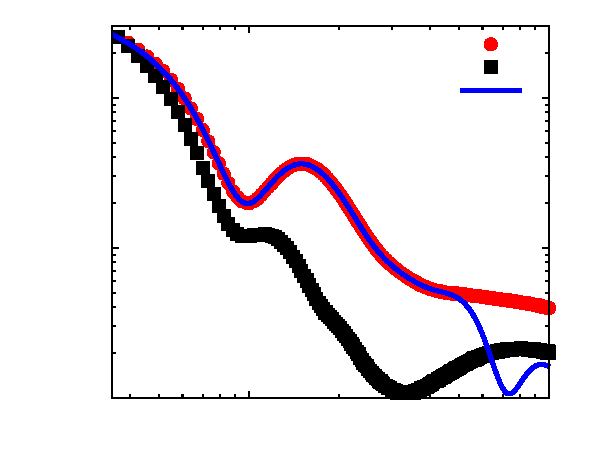
\includegraphics{CaelyxIodixanolSingleContrast}}%
    \gplfronttext
  \end{picture}%
\endgroup

		\caption{Caelyx in buffer and in 9.1 $\%$ iodixanol: SAXS scattering curve at single contrast compared to that of an SSL of similar size}
		\label{fig:CaelyxIodixanolSingleContrast}
\end{figure}

\subsection{Iso-osmolar contrast agent: Iodixinol}
\subsection{Sterically Stabilized Liposomes (SSLs) of different sizes}
\subsection{Lipoproteins}
HDL and LDL

\section{Traceable size determination of a liposomal drug}
SAXS curves of the liposomal doxorubicin sample measured at different suspending medium electron densities are shown in Fig. 1. In the scattering curves, it is possible to observe the variation of the curve features through the increase of the suspending medium density, which indicates the complexity of the internal structure of the nanocarrier. Besides, the appearance of an intersection point around q = 0.12 nm$^{-1}$ is a further indicator of the structural complexity of the drug-carrier.

\begin{figure}
	\centering
		\subfloat[Contrast variation with density gradient]{\resizebox{0.44\linewidth}{!}{% GNUPLOT: LaTeX picture with Postscript
\begingroup
  \makeatletter
  \providecommand\color[2][]{%
    \GenericError{(gnuplot) \space\space\space\@spaces}{%
      Package color not loaded in conjunction with
      terminal option `colourtext'%
    }{See the gnuplot documentation for explanation.%
    }{Either use 'blacktext' in gnuplot or load the package
      color.sty in LaTeX.}%
    \renewcommand\color[2][]{}%
  }%
  \providecommand\includegraphics[2][]{%
    \GenericError{(gnuplot) \space\space\space\@spaces}{%
      Package graphicx or graphics not loaded%
    }{See the gnuplot documentation for explanation.%
    }{The gnuplot epslatex terminal needs graphicx.sty or graphics.sty.}%
    \renewcommand\includegraphics[2][]{}%
  }%
  \providecommand\rotatebox[2]{#2}%
  \@ifundefined{ifGPcolor}{%
    \newif\ifGPcolor
    \GPcolortrue
  }{}%
  \@ifundefined{ifGPblacktext}{%
    \newif\ifGPblacktext
    \GPblacktextfalse
  }{}%
  % define a \g@addto@macro without @ in the name:
  \let\gplgaddtomacro\g@addto@macro
  % define empty templates for all commands taking text:
  \gdef\gplbacktext{}%
  \gdef\gplfronttext{}%
  \makeatother
  \ifGPblacktext
    % no textcolor at all
    \def\colorrgb#1{}%
    \def\colorgray#1{}%
  \else
    % gray or color?
    \ifGPcolor
      \def\colorrgb#1{\color[rgb]{#1}}%
      \def\colorgray#1{\color[gray]{#1}}%
      \expandafter\def\csname LTw\endcsname{\color{white}}%
      \expandafter\def\csname LTb\endcsname{\color{black}}%
      \expandafter\def\csname LTa\endcsname{\color{black}}%
      \expandafter\def\csname LT0\endcsname{\color[rgb]{1,0,0}}%
      \expandafter\def\csname LT1\endcsname{\color[rgb]{0,1,0}}%
      \expandafter\def\csname LT2\endcsname{\color[rgb]{0,0,1}}%
      \expandafter\def\csname LT3\endcsname{\color[rgb]{1,0,1}}%
      \expandafter\def\csname LT4\endcsname{\color[rgb]{0,1,1}}%
      \expandafter\def\csname LT5\endcsname{\color[rgb]{1,1,0}}%
      \expandafter\def\csname LT6\endcsname{\color[rgb]{0,0,0}}%
      \expandafter\def\csname LT7\endcsname{\color[rgb]{1,0.3,0}}%
      \expandafter\def\csname LT8\endcsname{\color[rgb]{0.5,0.5,0.5}}%
    \else
      % gray
      \def\colorrgb#1{\color{black}}%
      \def\colorgray#1{\color[gray]{#1}}%
      \expandafter\def\csname LTw\endcsname{\color{white}}%
      \expandafter\def\csname LTb\endcsname{\color{black}}%
      \expandafter\def\csname LTa\endcsname{\color{black}}%
      \expandafter\def\csname LT0\endcsname{\color{black}}%
      \expandafter\def\csname LT1\endcsname{\color{black}}%
      \expandafter\def\csname LT2\endcsname{\color{black}}%
      \expandafter\def\csname LT3\endcsname{\color{black}}%
      \expandafter\def\csname LT4\endcsname{\color{black}}%
      \expandafter\def\csname LT5\endcsname{\color{black}}%
      \expandafter\def\csname LT6\endcsname{\color{black}}%
      \expandafter\def\csname LT7\endcsname{\color{black}}%
      \expandafter\def\csname LT8\endcsname{\color{black}}%
    \fi
  \fi
    \setlength{\unitlength}{0.0500bp}%
    \ifx\gptboxheight\undefined%
      \newlength{\gptboxheight}%
      \newlength{\gptboxwidth}%
      \newsavebox{\gptboxtext}%
    \fi%
    \setlength{\fboxrule}{0.5pt}%
    \setlength{\fboxsep}{1pt}%
\begin{picture}(5668.00,4534.00)%
    \gplgaddtomacro\gplbacktext{%
      \csname LTb\endcsname%
      \put(814,1234){\makebox(0,0)[r]{\strut{}$0.01$}}%
      \csname LTb\endcsname%
      \put(814,1993){\makebox(0,0)[r]{\strut{}$0.1$}}%
      \csname LTb\endcsname%
      \put(814,2752){\makebox(0,0)[r]{\strut{}$1$}}%
      \csname LTb\endcsname%
      \put(814,3510){\makebox(0,0)[r]{\strut{}$10$}}%
      \csname LTb\endcsname%
      \put(814,4269){\makebox(0,0)[r]{\strut{}$100$}}%
      \csname LTb\endcsname%
      \put(1453,484){\makebox(0,0){\strut{}$0.05$}}%
      \csname LTb\endcsname%
      \put(2142,484){\makebox(0,0){\strut{}$0.1$}}%
      \csname LTb\endcsname%
      \put(2830,484){\makebox(0,0){\strut{}$0.2$}}%
      \csname LTb\endcsname%
      \put(3741,484){\makebox(0,0){\strut{}$0.5$}}%
      \csname LTb\endcsname%
      \put(4429,484){\makebox(0,0){\strut{}$1$}}%
    }%
    \gplgaddtomacro\gplfronttext{%
      \csname LTb\endcsname%
      \put(176,2266){\rotatebox{-270}{\makebox(0,0){\strut{}Scattering Intensity / cm$^{-1}$}}}%
      \put(2687,154){\makebox(0,0){\strut{}$q$ / nm$^{-1}$}}%
      \csname LTb\endcsname%
      \put(4691,1149){\makebox(0,0)[l]{\strut{}\smaller 345}}%
      \put(4691,1892){\makebox(0,0)[l]{\strut{}\smaller 350}}%
      \put(4691,2635){\makebox(0,0)[l]{\strut{}\smaller 355}}%
      \put(4691,3377){\makebox(0,0)[l]{\strut{}\smaller 360}}%
      \put(4691,4120){\makebox(0,0)[l]{\strut{}\smaller 365}}%
      \put(5351,2486){\rotatebox{-90}{\makebox(0,0){\strut{}\smaller Solvent Electron Density / nm$^{-3}$}}}%
    }%
    \gplbacktext
    \put(0,0){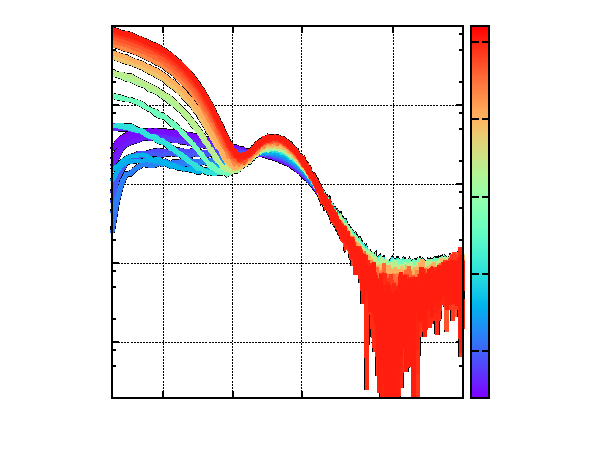
\includegraphics{CaelyxIodixanolContinuousSAXS}}%
    \gplfronttext
  \end{picture}%
\endgroup
}\label{fig:CaelyxIodixanolContinuousSAXS}}
		\subfloat[Isoscattering point positions]{\resizebox{0.44\linewidth}{!}{% GNUPLOT: LaTeX picture with Postscript
\begingroup
  \makeatletter
  \providecommand\color[2][]{%
    \GenericError{(gnuplot) \space\space\space\@spaces}{%
      Package color not loaded in conjunction with
      terminal option `colourtext'%
    }{See the gnuplot documentation for explanation.%
    }{Either use 'blacktext' in gnuplot or load the package
      color.sty in LaTeX.}%
    \renewcommand\color[2][]{}%
  }%
  \providecommand\includegraphics[2][]{%
    \GenericError{(gnuplot) \space\space\space\@spaces}{%
      Package graphicx or graphics not loaded%
    }{See the gnuplot documentation for explanation.%
    }{The gnuplot epslatex terminal needs graphicx.sty or graphics.sty.}%
    \renewcommand\includegraphics[2][]{}%
  }%
  \providecommand\rotatebox[2]{#2}%
  \@ifundefined{ifGPcolor}{%
    \newif\ifGPcolor
    \GPcolortrue
  }{}%
  \@ifundefined{ifGPblacktext}{%
    \newif\ifGPblacktext
    \GPblacktextfalse
  }{}%
  % define a \g@addto@macro without @ in the name:
  \let\gplgaddtomacro\g@addto@macro
  % define empty templates for all commands taking text:
  \gdef\gplbacktext{}%
  \gdef\gplfronttext{}%
  \makeatother
  \ifGPblacktext
    % no textcolor at all
    \def\colorrgb#1{}%
    \def\colorgray#1{}%
  \else
    % gray or color?
    \ifGPcolor
      \def\colorrgb#1{\color[rgb]{#1}}%
      \def\colorgray#1{\color[gray]{#1}}%
      \expandafter\def\csname LTw\endcsname{\color{white}}%
      \expandafter\def\csname LTb\endcsname{\color{black}}%
      \expandafter\def\csname LTa\endcsname{\color{black}}%
      \expandafter\def\csname LT0\endcsname{\color[rgb]{1,0,0}}%
      \expandafter\def\csname LT1\endcsname{\color[rgb]{0,1,0}}%
      \expandafter\def\csname LT2\endcsname{\color[rgb]{0,0,1}}%
      \expandafter\def\csname LT3\endcsname{\color[rgb]{1,0,1}}%
      \expandafter\def\csname LT4\endcsname{\color[rgb]{0,1,1}}%
      \expandafter\def\csname LT5\endcsname{\color[rgb]{1,1,0}}%
      \expandafter\def\csname LT6\endcsname{\color[rgb]{0,0,0}}%
      \expandafter\def\csname LT7\endcsname{\color[rgb]{1,0.3,0}}%
      \expandafter\def\csname LT8\endcsname{\color[rgb]{0.5,0.5,0.5}}%
    \else
      % gray
      \def\colorrgb#1{\color{black}}%
      \def\colorgray#1{\color[gray]{#1}}%
      \expandafter\def\csname LTw\endcsname{\color{white}}%
      \expandafter\def\csname LTb\endcsname{\color{black}}%
      \expandafter\def\csname LTa\endcsname{\color{black}}%
      \expandafter\def\csname LT0\endcsname{\color{black}}%
      \expandafter\def\csname LT1\endcsname{\color{black}}%
      \expandafter\def\csname LT2\endcsname{\color{black}}%
      \expandafter\def\csname LT3\endcsname{\color{black}}%
      \expandafter\def\csname LT4\endcsname{\color{black}}%
      \expandafter\def\csname LT5\endcsname{\color{black}}%
      \expandafter\def\csname LT6\endcsname{\color{black}}%
      \expandafter\def\csname LT7\endcsname{\color{black}}%
      \expandafter\def\csname LT8\endcsname{\color{black}}%
    \fi
  \fi
  \setlength{\unitlength}{0.0500bp}%
  \begin{picture}(5668.00,4534.00)%
    \gplgaddtomacro\gplbacktext{%
      \csname LTb\endcsname%
      \put(814,2055){\makebox(0,0)[r]{\strut{} 0.1}}%
      \csname LTb\endcsname%
      \put(814,3987){\makebox(0,0)[r]{\strut{} 1}}%
      \csname LTb\endcsname%
      \put(946,484){\makebox(0,0){\strut{} 0.05}}%
      \csname LTb\endcsname%
      \put(1947,484){\makebox(0,0){\strut{} 0.1}}%
      \csname LTb\endcsname%
      \put(2947,484){\makebox(0,0){\strut{} 0.2}}%
      \csname LTb\endcsname%
      \put(4270,484){\makebox(0,0){\strut{} 0.5}}%
      \csname LTb\endcsname%
      \put(5271,484){\makebox(0,0){\strut{} 1}}%
      \put(176,2266){\rotatebox{-270}{\makebox(0,0){\strut{}Rel. Std. Deviation}}}%
      \put(3108,154){\makebox(0,0){\strut{}$q$ / nm$^{-1}$}}%
    }%
    \gplgaddtomacro\gplfronttext{%
      \csname LTb\endcsname%
      \put(4548,4041){\makebox(0,0)[r]{\strut{}\smaller Background subtracted}}%
      \csname LTb\endcsname%
      \put(4548,3711){\makebox(0,0)[r]{\strut{}\smaller Raw data}}%
    }%
    \gplbacktext
    \put(0,0){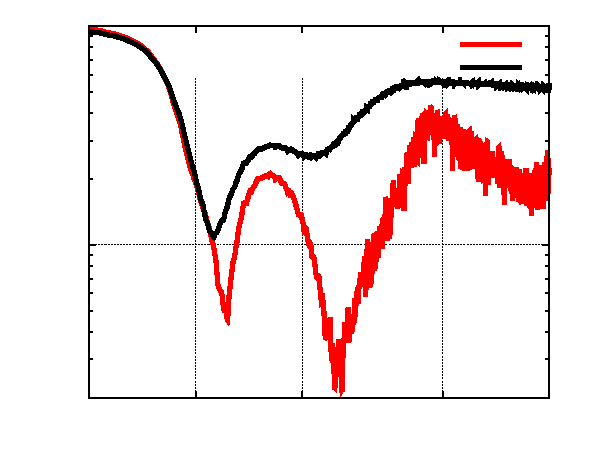
\includegraphics{CaelyxIodixanolIsopoint}}%
    \gplfronttext
  \end{picture}%
\endgroup
}\label{fig:CaelyxIodixanolIsopoint}}
		\caption{Scattering curves at different suspending medium electron densities obtained with a solvent density gradient of Caelyx in aqueous iodixanol with constant buffer osmolality. The inset shows the precise position of the isoscattering points}
\end{figure}

The solvent background has been subtracted by measuring the scattering curves of a density gradient of Optiprep® and buffer without nanocarriers. The low scattering power of the PEGylated liposomal doxorubicin at high q values and the contribution of the iodixanol background  result in an increased uncertainty in the high-q range of the corrected scattering curves, although in the Fourier region below q = 0.3 nm$^{-1}$ the background effect is almost negligible.

\subsection{Isoscattering point approach}
In the low $q$ part of the scattering curve, an isoscattering point is clearly visible as highlighted in Fig.1, where all the scattering curves intersect at one point. The isoscattering point position relates directly to the external radius of the measured particle inaccessible to the solvent, as explained in the Supplementary Information. Therefore, the PEG-chains attached to the liposome surface might not be quantified in this approach due to the permeability of the polymer layer. The isoscattering point position is precisely determined by calculating the relative standard deviation of all the scattering curves at each q-value, as shown in the inset of Fig.1. The first isoscattering point $q^{\star}_1$ is located at $q^{\star}_1 = 0.123$ nm$^{-1}$, which corresponds to a radius of $R = 36.5$ nm and a diameter of 73 nm. A second isoscattering point at q*2 = 0.25 nm-1 is still visible, although the diffuseness of the isoscattering points at higher q values, related with the polydispersity of the ensemble, makes it less reliable for the determination of the outer radius.

The determination of the $q$ values have an associated relative uncertainty of 0.1 $\%$, which corresponds to a size uncertainty of 0.6 nm. Furthermore, the radial integration of the scattering pattern was performed choosing a $q$-bin of size 0.0015 nm$^{-1}$, with an associated uncertainty in the size of 0.9 nm. Without further considerations, the Caelyx$\textregistered$ size uncertainty associated to the determination of the $q$-value of the isoscattering point is 1.1 nm. Other possible sources of uncertainty arise from the polydispersity degree of the sample and the ellipticity of the doxorubicin loaded liposomes, which might shift the measured position of the isoscattering point, although the uncertainty associated to them cannot be easily quantified. 

\subsection{Shape factor calculation}
In order to provide a traceable uncertainty for the obtained size value, we have used an alternative evaluation procedure, namely the calculation of the so-called shape factor which extracts all contributions from the 30 measured scattering curves that change with the contrast at different solvent densities. The shape factor of the Caelyx$\textregistered$ sample contains essentially information only about the shape and size distribution of the space filled up by the liposomes, i.e. the contributions of the phospholipid bilayer and the encapsulated doxorubicin to the scattering intensity are cancelled.  Thus, the complex interpretation of the original SAXS curve of Caelyx$\textregistered$ is avoided and enables the size determination of the liposomal carrier by fitting a simple analytical model for homogeneous spherical objects. A model with a certain ellipticity was also attempted, due to the slight liposomal eccentricity observed in TEM images though the best fit was accomplished with a spherical model. Details on the calculation of the shape factor as well as the analytical expression for the model fitting can be found in the Supplementary Information. 

\begin{figure}
	\centering
		% GNUPLOT: LaTeX picture with Postscript
\begingroup
  \makeatletter
  \providecommand\color[2][]{%
    \GenericError{(gnuplot) \space\space\space\@spaces}{%
      Package color not loaded in conjunction with
      terminal option `colourtext'%
    }{See the gnuplot documentation for explanation.%
    }{Either use 'blacktext' in gnuplot or load the package
      color.sty in LaTeX.}%
    \renewcommand\color[2][]{}%
  }%
  \providecommand\includegraphics[2][]{%
    \GenericError{(gnuplot) \space\space\space\@spaces}{%
      Package graphicx or graphics not loaded%
    }{See the gnuplot documentation for explanation.%
    }{The gnuplot epslatex terminal needs graphicx.sty or graphics.sty.}%
    \renewcommand\includegraphics[2][]{}%
  }%
  \providecommand\rotatebox[2]{#2}%
  \@ifundefined{ifGPcolor}{%
    \newif\ifGPcolor
    \GPcolortrue
  }{}%
  \@ifundefined{ifGPblacktext}{%
    \newif\ifGPblacktext
    \GPblacktextfalse
  }{}%
  % define a \g@addto@macro without @ in the name:
  \let\gplgaddtomacro\g@addto@macro
  % define empty templates for all commands taking text:
  \gdef\gplbacktext{}%
  \gdef\gplfronttext{}%
  \makeatother
  \ifGPblacktext
    % no textcolor at all
    \def\colorrgb#1{}%
    \def\colorgray#1{}%
  \else
    % gray or color?
    \ifGPcolor
      \def\colorrgb#1{\color[rgb]{#1}}%
      \def\colorgray#1{\color[gray]{#1}}%
      \expandafter\def\csname LTw\endcsname{\color{white}}%
      \expandafter\def\csname LTb\endcsname{\color{black}}%
      \expandafter\def\csname LTa\endcsname{\color{black}}%
      \expandafter\def\csname LT0\endcsname{\color[rgb]{1,0,0}}%
      \expandafter\def\csname LT1\endcsname{\color[rgb]{0,1,0}}%
      \expandafter\def\csname LT2\endcsname{\color[rgb]{0,0,1}}%
      \expandafter\def\csname LT3\endcsname{\color[rgb]{1,0,1}}%
      \expandafter\def\csname LT4\endcsname{\color[rgb]{0,1,1}}%
      \expandafter\def\csname LT5\endcsname{\color[rgb]{1,1,0}}%
      \expandafter\def\csname LT6\endcsname{\color[rgb]{0,0,0}}%
      \expandafter\def\csname LT7\endcsname{\color[rgb]{1,0.3,0}}%
      \expandafter\def\csname LT8\endcsname{\color[rgb]{0.5,0.5,0.5}}%
    \else
      % gray
      \def\colorrgb#1{\color{black}}%
      \def\colorgray#1{\color[gray]{#1}}%
      \expandafter\def\csname LTw\endcsname{\color{white}}%
      \expandafter\def\csname LTb\endcsname{\color{black}}%
      \expandafter\def\csname LTa\endcsname{\color{black}}%
      \expandafter\def\csname LT0\endcsname{\color{black}}%
      \expandafter\def\csname LT1\endcsname{\color{black}}%
      \expandafter\def\csname LT2\endcsname{\color{black}}%
      \expandafter\def\csname LT3\endcsname{\color{black}}%
      \expandafter\def\csname LT4\endcsname{\color{black}}%
      \expandafter\def\csname LT5\endcsname{\color{black}}%
      \expandafter\def\csname LT6\endcsname{\color{black}}%
      \expandafter\def\csname LT7\endcsname{\color{black}}%
      \expandafter\def\csname LT8\endcsname{\color{black}}%
    \fi
  \fi
  \setlength{\unitlength}{0.0500bp}%
  \begin{picture}(5668.00,4534.00)%
    \gplgaddtomacro\gplbacktext{%
      \csname LTb\endcsname%
      \put(990,704){\makebox(0,0)[r]{\strut{} 1}}%
      \csname LTb\endcsname%
      \put(990,1595){\makebox(0,0)[r]{\strut{} 10}}%
      \csname LTb\endcsname%
      \put(990,2487){\makebox(0,0)[r]{\strut{} 100}}%
      \csname LTb\endcsname%
      \put(990,3378){\makebox(0,0)[r]{\strut{} 1000}}%
      \csname LTb\endcsname%
      \put(990,4269){\makebox(0,0)[r]{\strut{} 10000}}%
      \csname LTb\endcsname%
      \put(2279,484){\makebox(0,0){\strut{} 0.05}}%
      \csname LTb\endcsname%
      \put(3437,484){\makebox(0,0){\strut{} 0.1}}%
      \csname LTb\endcsname%
      \put(4594,484){\makebox(0,0){\strut{} 0.2}}%
      \csname LTb\endcsname%
      \put(5271,484){\makebox(0,0){\strut{} 0.3}}%
      \put(220,2486){\rotatebox{-270}{\makebox(0,0){\strut{}Shape Factor / a.u.}}}%
      \put(3196,154){\makebox(0,0){\strut{}$q$ / nm$^{-1}$}}%
    }%
    \gplgaddtomacro\gplfronttext{%
      \csname LTb\endcsname%
      \put(4284,4010){\makebox(0,0)[r]{\strut{}Experimental Data}}%
      \csname LTb\endcsname%
      \put(4284,3617){\makebox(0,0)[r]{\strut{}Sphere Fit}}%
    }%
    \gplbacktext
    \put(0,0){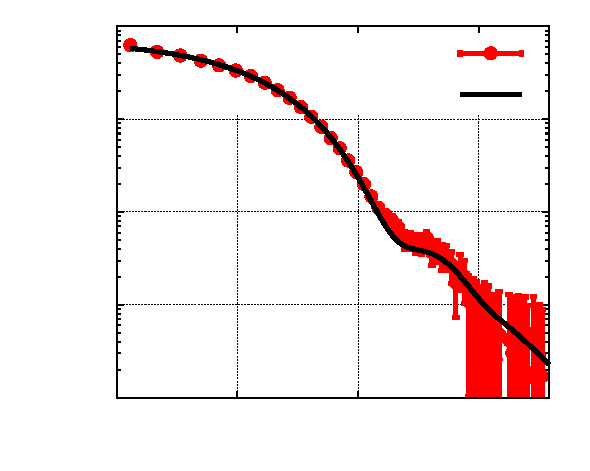
\includegraphics{CaelyxIodixanolResonantTerm}}%
    \gplfronttext
  \end{picture}%
\endgroup

		\caption{Shape factor of the liposomes obtained from the experimental data is shown with black circles and the model fit for homogeneous spherical particles is depicted in red.}
		\label{fig:CaelyxIodixanolResonantTerm}
\end{figure}

The shape factor calculated from the SAXS curves and the theoretical model fitting are depicted in Fig. 2. The mean diameter obtained from the spherical form factor fit is (65.5 $\pm$ 4.7) nm, slightly smaller than the value calculated from the isoscattering point position. Nevertheless, both values overlap when considering the associated standard uncertainties and that the polydispersity smearing of the isoscattering point is difficult to quantify. The latter fact is supported by the broad size distribution determined by the shape factor fitting. When assuming a Gaussian size distribution, the polydispersity degree (defined as the full width at half maximum of the size distribution divided by its mean value) of the nanocarrier is ca. 40$\%$. Therefore, the average value of (69 $\pm$ 5) nm can be embraced as a reliable external size for the liposomal drug-carrier.

The average size obtained by contrast variation in SAXS is smaller than the result obtained with DLS of ca. 86 nm (in-house measurement), which can be attributed to the fact that the DLS measurand is the hydrodynamic size of the nanoparticles, while SAXS provides the size of the spherical volume inaccessible to the solvent. As the 2 kDa PEG-chains attached to the surface of the liposomes contribute to the hydrodynamic radius but that layer is permeable to the solvent and, therefore, invisible to contrast variation SAXS, the ca. 15 nm difference between the sizes determined by DLS and SAXS is justified. 

\subsection{Average electron density}
At low $q$-values, the Guinier approximation can be used as explained in the Supplementary Information. By fitting the spherical form factor to the q-range just below the first minimum of the scattering curves, an extrapolated value for the intensity at zero-angle I(0) could be obtained as displayed in Fig. 3. The minimum of the parabola fitted to the experimental points determines the average electron density of the drug carrier system, according to the equation $I(0) \propto (\rho_0-\rho_{solv})^2$.

\begin{figure}
	\centering
		% GNUPLOT: LaTeX picture with Postscript
\begingroup
  \makeatletter
  \providecommand\color[2][]{%
    \GenericError{(gnuplot) \space\space\space\@spaces}{%
      Package color not loaded in conjunction with
      terminal option `colourtext'%
    }{See the gnuplot documentation for explanation.%
    }{Either use 'blacktext' in gnuplot or load the package
      color.sty in LaTeX.}%
    \renewcommand\color[2][]{}%
  }%
  \providecommand\includegraphics[2][]{%
    \GenericError{(gnuplot) \space\space\space\@spaces}{%
      Package graphicx or graphics not loaded%
    }{See the gnuplot documentation for explanation.%
    }{The gnuplot epslatex terminal needs graphicx.sty or graphics.sty.}%
    \renewcommand\includegraphics[2][]{}%
  }%
  \providecommand\rotatebox[2]{#2}%
  \@ifundefined{ifGPcolor}{%
    \newif\ifGPcolor
    \GPcolortrue
  }{}%
  \@ifundefined{ifGPblacktext}{%
    \newif\ifGPblacktext
    \GPblacktextfalse
  }{}%
  % define a \g@addto@macro without @ in the name:
  \let\gplgaddtomacro\g@addto@macro
  % define empty templates for all commands taking text:
  \gdef\gplbacktext{}%
  \gdef\gplfronttext{}%
  \makeatother
  \ifGPblacktext
    % no textcolor at all
    \def\colorrgb#1{}%
    \def\colorgray#1{}%
  \else
    % gray or color?
    \ifGPcolor
      \def\colorrgb#1{\color[rgb]{#1}}%
      \def\colorgray#1{\color[gray]{#1}}%
      \expandafter\def\csname LTw\endcsname{\color{white}}%
      \expandafter\def\csname LTb\endcsname{\color{black}}%
      \expandafter\def\csname LTa\endcsname{\color{black}}%
      \expandafter\def\csname LT0\endcsname{\color[rgb]{1,0,0}}%
      \expandafter\def\csname LT1\endcsname{\color[rgb]{0,1,0}}%
      \expandafter\def\csname LT2\endcsname{\color[rgb]{0,0,1}}%
      \expandafter\def\csname LT3\endcsname{\color[rgb]{1,0,1}}%
      \expandafter\def\csname LT4\endcsname{\color[rgb]{0,1,1}}%
      \expandafter\def\csname LT5\endcsname{\color[rgb]{1,1,0}}%
      \expandafter\def\csname LT6\endcsname{\color[rgb]{0,0,0}}%
      \expandafter\def\csname LT7\endcsname{\color[rgb]{1,0.3,0}}%
      \expandafter\def\csname LT8\endcsname{\color[rgb]{0.5,0.5,0.5}}%
    \else
      % gray
      \def\colorrgb#1{\color{black}}%
      \def\colorgray#1{\color[gray]{#1}}%
      \expandafter\def\csname LTw\endcsname{\color{white}}%
      \expandafter\def\csname LTb\endcsname{\color{black}}%
      \expandafter\def\csname LTa\endcsname{\color{black}}%
      \expandafter\def\csname LT0\endcsname{\color{black}}%
      \expandafter\def\csname LT1\endcsname{\color{black}}%
      \expandafter\def\csname LT2\endcsname{\color{black}}%
      \expandafter\def\csname LT3\endcsname{\color{black}}%
      \expandafter\def\csname LT4\endcsname{\color{black}}%
      \expandafter\def\csname LT5\endcsname{\color{black}}%
      \expandafter\def\csname LT6\endcsname{\color{black}}%
      \expandafter\def\csname LT7\endcsname{\color{black}}%
      \expandafter\def\csname LT8\endcsname{\color{black}}%
    \fi
  \fi
    \setlength{\unitlength}{0.0500bp}%
    \ifx\gptboxheight\undefined%
      \newlength{\gptboxheight}%
      \newlength{\gptboxwidth}%
      \newsavebox{\gptboxtext}%
    \fi%
    \setlength{\fboxrule}{0.5pt}%
    \setlength{\fboxsep}{1pt}%
\begin{picture}(5668.00,4534.00)%
    \gplgaddtomacro\gplbacktext{%
      \csname LTb\endcsname%
      \put(814,704){\makebox(0,0)[r]{\strut{}$0$}}%
      \csname LTb\endcsname%
      \put(814,1274){\makebox(0,0)[r]{\strut{}$20$}}%
      \csname LTb\endcsname%
      \put(814,1845){\makebox(0,0)[r]{\strut{}$40$}}%
      \csname LTb\endcsname%
      \put(814,2415){\makebox(0,0)[r]{\strut{}$60$}}%
      \csname LTb\endcsname%
      \put(814,2986){\makebox(0,0)[r]{\strut{}$80$}}%
      \csname LTb\endcsname%
      \put(814,3556){\makebox(0,0)[r]{\strut{}$100$}}%
      \csname LTb\endcsname%
      \put(814,4126){\makebox(0,0)[r]{\strut{}$120$}}%
      \csname LTb\endcsname%
      \put(1510,484){\makebox(0,0){\strut{}$345$}}%
      \csname LTb\endcsname%
      \put(2450,484){\makebox(0,0){\strut{}$350$}}%
      \csname LTb\endcsname%
      \put(3391,484){\makebox(0,0){\strut{}$355$}}%
      \csname LTb\endcsname%
      \put(4331,484){\makebox(0,0){\strut{}$360$}}%
      \csname LTb\endcsname%
      \put(5271,484){\makebox(0,0){\strut{}$365$}}%
    }%
    \gplgaddtomacro\gplfronttext{%
      \csname LTb\endcsname%
      \put(176,2486){\rotatebox{-270}{\makebox(0,0){\strut{}$I(0)$ / cm$^{-1}$}}}%
      \put(3108,154){\makebox(0,0){\strut{}Solvent Electron Density / nm$^{-3}$}}%
    }%
    \gplbacktext
    \put(0,0){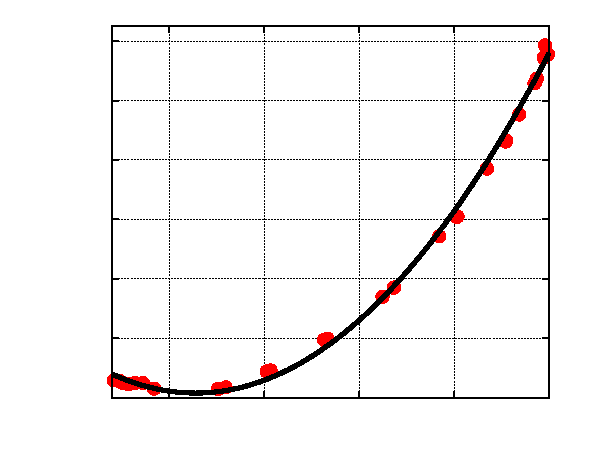
\includegraphics{CaelyxAverageDensity}}%
    \gplfronttext
  \end{picture}%
\endgroup

		\caption{Measured intensity at zero-angle of Caelyx as a function of the electron density of the aqueous iodixanol suspending medium. The function fitted to the experimental data is depicted in black: Average density is 346.39 nm$^{-3}$ and there is a offset of 1.56 cm$^{-1}$}
		\label{fig:CaelyxAverageDensity}
\end{figure}

From this calculation, a value of $\rho_0$ = (346.2 $\pm$ 1.2) nm$^{-3}$ is obtained which corresponds to the density of the liposomal nanocarrier and the precipitated drug combined. The uncertainty of 1.2 nm$^{-3}$ is associated with the vertical size of the focused X-ray beam. The obtained density is slightly higher than the value of 338 nm$^{-3}$ estimated for empty PEGylated liposomes due to the presence of the doxorubicin-sulfate aggregate in the intraliposomal volume. 

Due to the constant osmolality of the suspending medium along the whole density gradient, no osmotic pressure effects were observed in the size or density of the liposomal system. Nevertheless, the importance of the buffer osmotic effects in the liposomal structure cannot be neglected and a thorough study will be discussed in the following section.

\section{Osmotic effects in liposomes}
\subsection{Application to drug-stabilized liposomes}
The osmotic behavior of liposomes depends, basically, on their size and chemical composition. Larger liposomes tend to be osmotically activeand, in this case, intraliposomal osmolality should be equal to the buffer outside of the liposomes. Nevertheless, the small size of Caelyx® and the doxorubicin-sulfate aggregate in the intraliposomal volume create an extraordinary resistance against the buffer osmotic pressure. This effect can be studied by increasing systematically the osmolality of the suspending medium, e.g. increasing the sucrose concentration in the aqueous buffer.

\begin{figure}
	\centering
		\subfloat[Osmotic effects in Caelys by using sucrose as contrast agent]{\resizebox{0.44\linewidth}{!}{% GNUPLOT: LaTeX picture with Postscript
\begingroup
  \makeatletter
  \providecommand\color[2][]{%
    \GenericError{(gnuplot) \space\space\space\@spaces}{%
      Package color not loaded in conjunction with
      terminal option `colourtext'%
    }{See the gnuplot documentation for explanation.%
    }{Either use 'blacktext' in gnuplot or load the package
      color.sty in LaTeX.}%
    \renewcommand\color[2][]{}%
  }%
  \providecommand\includegraphics[2][]{%
    \GenericError{(gnuplot) \space\space\space\@spaces}{%
      Package graphicx or graphics not loaded%
    }{See the gnuplot documentation for explanation.%
    }{The gnuplot epslatex terminal needs graphicx.sty or graphics.sty.}%
    \renewcommand\includegraphics[2][]{}%
  }%
  \providecommand\rotatebox[2]{#2}%
  \@ifundefined{ifGPcolor}{%
    \newif\ifGPcolor
    \GPcolortrue
  }{}%
  \@ifundefined{ifGPblacktext}{%
    \newif\ifGPblacktext
    \GPblacktextfalse
  }{}%
  % define a \g@addto@macro without @ in the name:
  \let\gplgaddtomacro\g@addto@macro
  % define empty templates for all commands taking text:
  \gdef\gplbacktext{}%
  \gdef\gplfronttext{}%
  \makeatother
  \ifGPblacktext
    % no textcolor at all
    \def\colorrgb#1{}%
    \def\colorgray#1{}%
  \else
    % gray or color?
    \ifGPcolor
      \def\colorrgb#1{\color[rgb]{#1}}%
      \def\colorgray#1{\color[gray]{#1}}%
      \expandafter\def\csname LTw\endcsname{\color{white}}%
      \expandafter\def\csname LTb\endcsname{\color{black}}%
      \expandafter\def\csname LTa\endcsname{\color{black}}%
      \expandafter\def\csname LT0\endcsname{\color[rgb]{1,0,0}}%
      \expandafter\def\csname LT1\endcsname{\color[rgb]{0,1,0}}%
      \expandafter\def\csname LT2\endcsname{\color[rgb]{0,0,1}}%
      \expandafter\def\csname LT3\endcsname{\color[rgb]{1,0,1}}%
      \expandafter\def\csname LT4\endcsname{\color[rgb]{0,1,1}}%
      \expandafter\def\csname LT5\endcsname{\color[rgb]{1,1,0}}%
      \expandafter\def\csname LT6\endcsname{\color[rgb]{0,0,0}}%
      \expandafter\def\csname LT7\endcsname{\color[rgb]{1,0.3,0}}%
      \expandafter\def\csname LT8\endcsname{\color[rgb]{0.5,0.5,0.5}}%
    \else
      % gray
      \def\colorrgb#1{\color{black}}%
      \def\colorgray#1{\color[gray]{#1}}%
      \expandafter\def\csname LTw\endcsname{\color{white}}%
      \expandafter\def\csname LTb\endcsname{\color{black}}%
      \expandafter\def\csname LTa\endcsname{\color{black}}%
      \expandafter\def\csname LT0\endcsname{\color{black}}%
      \expandafter\def\csname LT1\endcsname{\color{black}}%
      \expandafter\def\csname LT2\endcsname{\color{black}}%
      \expandafter\def\csname LT3\endcsname{\color{black}}%
      \expandafter\def\csname LT4\endcsname{\color{black}}%
      \expandafter\def\csname LT5\endcsname{\color{black}}%
      \expandafter\def\csname LT6\endcsname{\color{black}}%
      \expandafter\def\csname LT7\endcsname{\color{black}}%
      \expandafter\def\csname LT8\endcsname{\color{black}}%
    \fi
  \fi
  \setlength{\unitlength}{0.0500bp}%
  \begin{picture}(5668.00,4534.00)%
    \gplgaddtomacro\gplbacktext{%
      \csname LTb\endcsname%
      \put(814,1053){\makebox(0,0)[r]{\strut{} 0.1}}%
      \csname LTb\endcsname%
      \put(814,2210){\makebox(0,0)[r]{\strut{} 1}}%
      \csname LTb\endcsname%
      \put(814,3368){\makebox(0,0)[r]{\strut{} 10}}%
      \csname LTb\endcsname%
      \put(1434,484){\makebox(0,0){\strut{} 0.05}}%
      \csname LTb\endcsname%
      \put(2096,484){\makebox(0,0){\strut{} 0.1}}%
      \csname LTb\endcsname%
      \put(2758,484){\makebox(0,0){\strut{} 0.2}}%
      \csname LTb\endcsname%
      \put(3633,484){\makebox(0,0){\strut{} 0.5}}%
      \csname LTb\endcsname%
      \put(4295,484){\makebox(0,0){\strut{} 1}}%
      \put(176,2266){\rotatebox{-270}{\makebox(0,0){\strut{}Scattering Intensity / cm$^{-1}$}}}%
      \put(2687,154){\makebox(0,0){\strut{}$q$ / nm$^{-1}$}}%
    }%
    \gplgaddtomacro\gplfronttext{%
      \csname LTb\endcsname%
      \put(4822,778){\makebox(0,0)[l]{\strut{}\smaller 200}}%
      \put(4822,1149){\makebox(0,0)[l]{\strut{}\smaller 400}}%
      \put(4822,1520){\makebox(0,0)[l]{\strut{}\smaller 600}}%
      \put(4822,1892){\makebox(0,0)[l]{\strut{}\smaller 800}}%
      \put(4822,2263){\makebox(0,0)[l]{\strut{}\smaller 1000}}%
      \put(4822,2635){\makebox(0,0)[l]{\strut{}\smaller 1200}}%
      \put(4822,3006){\makebox(0,0)[l]{\strut{}\smaller 1400}}%
      \put(4822,3377){\makebox(0,0)[l]{\strut{}\smaller 1600}}%
      \put(4822,3749){\makebox(0,0)[l]{\strut{}\smaller 1800}}%
      \put(4822,4120){\makebox(0,0)[l]{\strut{}\smaller 2000}}%
      \put(5483,2486){\rotatebox{-90}{\makebox(0,0){\strut{}\smaller Solvent Osmolality / mOsm kg$^{-1}$}}}%
    }%
    \gplbacktext
    \put(0,0){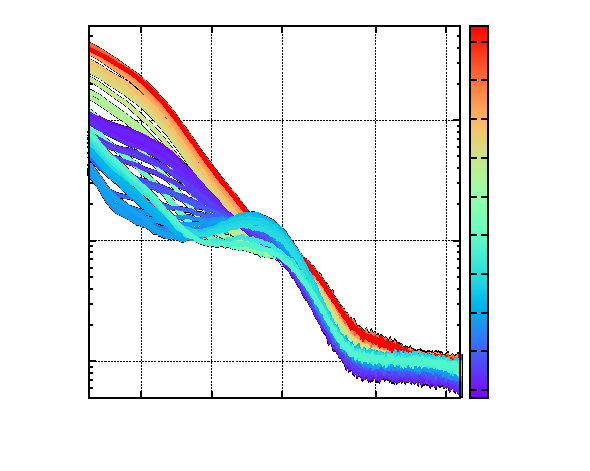
\includegraphics{CaelyxSucroseContinuousSAXS}}%
    \gplfronttext
  \end{picture}%
\endgroup
}\label{fig:CaelyxSucroseContinuousSAXS}}
		\subfloat[Isoscattering point intensity at 2 different setups: Osmotic threshold at 740 mOsm kg$^{-1}$]{\resizebox{0.44\linewidth}{!}{% GNUPLOT: LaTeX picture with Postscript
\begingroup
  \makeatletter
  \providecommand\color[2][]{%
    \GenericError{(gnuplot) \space\space\space\@spaces}{%
      Package color not loaded in conjunction with
      terminal option `colourtext'%
    }{See the gnuplot documentation for explanation.%
    }{Either use 'blacktext' in gnuplot or load the package
      color.sty in LaTeX.}%
    \renewcommand\color[2][]{}%
  }%
  \providecommand\includegraphics[2][]{%
    \GenericError{(gnuplot) \space\space\space\@spaces}{%
      Package graphicx or graphics not loaded%
    }{See the gnuplot documentation for explanation.%
    }{The gnuplot epslatex terminal needs graphicx.sty or graphics.sty.}%
    \renewcommand\includegraphics[2][]{}%
  }%
  \providecommand\rotatebox[2]{#2}%
  \@ifundefined{ifGPcolor}{%
    \newif\ifGPcolor
    \GPcolortrue
  }{}%
  \@ifundefined{ifGPblacktext}{%
    \newif\ifGPblacktext
    \GPblacktextfalse
  }{}%
  % define a \g@addto@macro without @ in the name:
  \let\gplgaddtomacro\g@addto@macro
  % define empty templates for all commands taking text:
  \gdef\gplbacktext{}%
  \gdef\gplfronttext{}%
  \makeatother
  \ifGPblacktext
    % no textcolor at all
    \def\colorrgb#1{}%
    \def\colorgray#1{}%
  \else
    % gray or color?
    \ifGPcolor
      \def\colorrgb#1{\color[rgb]{#1}}%
      \def\colorgray#1{\color[gray]{#1}}%
      \expandafter\def\csname LTw\endcsname{\color{white}}%
      \expandafter\def\csname LTb\endcsname{\color{black}}%
      \expandafter\def\csname LTa\endcsname{\color{black}}%
      \expandafter\def\csname LT0\endcsname{\color[rgb]{1,0,0}}%
      \expandafter\def\csname LT1\endcsname{\color[rgb]{0,1,0}}%
      \expandafter\def\csname LT2\endcsname{\color[rgb]{0,0,1}}%
      \expandafter\def\csname LT3\endcsname{\color[rgb]{1,0,1}}%
      \expandafter\def\csname LT4\endcsname{\color[rgb]{0,1,1}}%
      \expandafter\def\csname LT5\endcsname{\color[rgb]{1,1,0}}%
      \expandafter\def\csname LT6\endcsname{\color[rgb]{0,0,0}}%
      \expandafter\def\csname LT7\endcsname{\color[rgb]{1,0.3,0}}%
      \expandafter\def\csname LT8\endcsname{\color[rgb]{0.5,0.5,0.5}}%
    \else
      % gray
      \def\colorrgb#1{\color{black}}%
      \def\colorgray#1{\color[gray]{#1}}%
      \expandafter\def\csname LTw\endcsname{\color{white}}%
      \expandafter\def\csname LTb\endcsname{\color{black}}%
      \expandafter\def\csname LTa\endcsname{\color{black}}%
      \expandafter\def\csname LT0\endcsname{\color{black}}%
      \expandafter\def\csname LT1\endcsname{\color{black}}%
      \expandafter\def\csname LT2\endcsname{\color{black}}%
      \expandafter\def\csname LT3\endcsname{\color{black}}%
      \expandafter\def\csname LT4\endcsname{\color{black}}%
      \expandafter\def\csname LT5\endcsname{\color{black}}%
      \expandafter\def\csname LT6\endcsname{\color{black}}%
      \expandafter\def\csname LT7\endcsname{\color{black}}%
      \expandafter\def\csname LT8\endcsname{\color{black}}%
    \fi
  \fi
  \setlength{\unitlength}{0.0500bp}%
  \begin{picture}(5668.00,4534.00)%
    \gplgaddtomacro\gplbacktext{%
      \csname LTb\endcsname%
      \put(176,2486){\rotatebox{-270}{\makebox(0,0){\strut{}Intensity at $q=0.123$ nm$^{-1}$ / cm$^{-1}$}}}%
      \put(3108,154){\makebox(0,0){\strut{}Solvent Osmolality / mOsm kg$^{-1}$}}%
    }%
    \gplgaddtomacro\gplfronttext{%
      \csname LTb\endcsname%
      \put(4788,1331){\makebox(0,0)[r]{\strut{}\smaller SAXS}}%
      \csname LTb\endcsname%
      \put(4788,1001){\makebox(0,0)[r]{\strut{}\smaller WAXS}}%
      \csname LTb\endcsname%
      \put(814,704){\makebox(0,0)[r]{\strut{} 0.8}}%
      \csname LTb\endcsname%
      \put(814,1100){\makebox(0,0)[r]{\strut{} 1}}%
      \csname LTb\endcsname%
      \put(814,1496){\makebox(0,0)[r]{\strut{} 1.2}}%
      \csname LTb\endcsname%
      \put(814,1892){\makebox(0,0)[r]{\strut{} 1.4}}%
      \csname LTb\endcsname%
      \put(814,2288){\makebox(0,0)[r]{\strut{} 1.6}}%
      \csname LTb\endcsname%
      \put(814,2685){\makebox(0,0)[r]{\strut{} 1.8}}%
      \csname LTb\endcsname%
      \put(814,3081){\makebox(0,0)[r]{\strut{} 2}}%
      \csname LTb\endcsname%
      \put(814,3477){\makebox(0,0)[r]{\strut{} 2.2}}%
      \csname LTb\endcsname%
      \put(814,3873){\makebox(0,0)[r]{\strut{} 2.4}}%
      \csname LTb\endcsname%
      \put(814,4269){\makebox(0,0)[r]{\strut{} 2.6}}%
      \csname LTb\endcsname%
      \put(1270,484){\makebox(0,0){\strut{} 300}}%
      \csname LTb\endcsname%
      \put(1919,484){\makebox(0,0){\strut{} 600}}%
      \csname LTb\endcsname%
      \put(2568,484){\makebox(0,0){\strut{} 900}}%
      \csname LTb\endcsname%
      \put(3217,484){\makebox(0,0){\strut{} 1200}}%
      \csname LTb\endcsname%
      \put(3865,484){\makebox(0,0){\strut{} 1500}}%
      \csname LTb\endcsname%
      \put(4514,484){\makebox(0,0){\strut{} 1800}}%
      \csname LTb\endcsname%
      \put(5163,484){\makebox(0,0){\strut{} 2100}}%
      \put(2287,3477){\makebox(0,0)[l]{\strut{}\smaller \shortstack{Osmotic\\shrinkage}}}%
      \put(1465,3477){\makebox(0,0){\strut{}\smaller \shortstack{Constant\\shape\\and size}}}%
    }%
    \gplbacktext
    \put(0,0){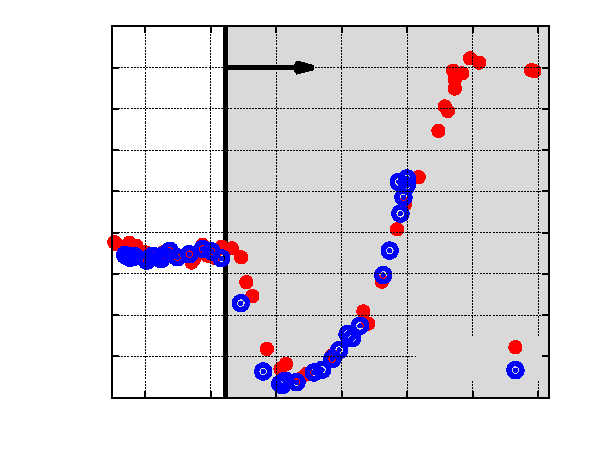
\includegraphics{CaelyxSucroseContinuousSAXSIsopoint}}%
    \gplfronttext
  \end{picture}%
\endgroup
}\label{fig:CaelyxSucroseContinuousSAXSIsopoint}}
		\caption{Scattering curves of Caelyx in an aqueous sucrose density gradient calibrated to the osmolality of the suspending medium. Intensity of the first isoscattering point depending on the aqueous sucrose solution osmolality is shown with black dots.}
\end{figure}

By means of the density gradient technique, scattering curves of the liposomal doxorubicin were recorded at different sucrose concentrations of the suspending medium, i.e. at different buffer osmolalities, as shown in Fig.4. The X-ray scattering measurements were performed at two different detector-to-sample distances, as described in the Materials and methods section, in order to study a broader $q$-range, spanning from 0.03 to 5.55 nm$^{-1}$, and observe the 1,0-diffraction peak of the doxorubicin fiber-like precipitate around $q=2.3$ nm$^{-1}$, as depicted in the inset of the Fig. 4 after proper background correction.

As discussed in the previous section, by increasing the electron density of the suspending medium, the scattering curves of the drug carrier change drastically due to contrast variation. In the case of the aqueous sucrose gradient shown in Fig. 4, this effect is also observed and strongly resembles the curves measured with the Optiprep TM density gradient depicted in Fig.1. Nevertheless, upon a certain sucrose concentration (reddish colored curves in Fig. 4), the features of the scattering curves disappear abruptly, because the suspending medium osmolality is so high that it induces morphological changes in the liposomal structure and, consequently, the scattering form factor of the particles changes.

This effect can be quantified by examining the intensity of the first isoscattering point at $q^{\star}_1 = 0.123$ nm$^{-1}$, because the scattered intensity at this point should be independent of the electron density of the solvent, as observed with the Optiprep TM gradient. The isoscattering point intensity as a function of the suspending medium osmolality is shown in Fig. 5 and there is a clear osmolality threshold at 670 mOsm kg$^{-1}$. Above this threshold, the osmotic pressure at the liposomal bilayer is so high that the liposome starts shrinking and changes its size, structure and, consequently, scattering form factor. The increased resistance against osmotic pressure, more than double the blood plasma osmolality and much higher than the osmolality needed to shrink empty PEGylated liposomes, is explained by the encapsulation of doxorubicin inside the liposome.

The large osmotic pressure produces a reversible shrinkage of the liposome though it is not capable of cracking it. This was proved in an additional experiment by increasing the osmolality of the buffer to 1333.6 mOsm kg$^{-1}$ with a sucrose mass fraction of 31.4$\%$ and then reducing it to 565.4 mOsm kg-1 by adding distilled water. The solvent with high osmolality produced a featureless scattering curve, as expected from Fig.4, whereas, after reducing the osmotic pressure, the scattering curve was the same as the measured Caelyx$\textregistered$ curve with the corresponding electron density, which gives evidence that the osmotic shrinkage process is reversible.

The behavior of the nano-drug for an increasing solvent osmolality can be further studied by evaluating the crystal structure of the doxorubicin aggregate, represented by the diffraction peak observed in the inset of figure Fig.4. The position of the peak in the reciprocal space depending on the suspending medium osmolality is depicted in Fig.5 and shows that its position deviates less than 1$\%$ from the weighted average $q=2.28$ nm$^{-1}$ along the whole osmolality range. This proves that the fiber-like structure of the drug inside the liposome is also constant during the osmotic shrinkage of the liposomes. The measured position of the (1,0) diffraction peak matches exactly the value measured from doxorubicin-sulfate complexes in solution.

\begin{figure}
	\centering
		\subfloat[Osmotic effects in Caelys by using sucrose as contrast agent]{\resizebox{0.44\linewidth}{!}{% GNUPLOT: LaTeX picture with Postscript
\begingroup
  \makeatletter
  \providecommand\color[2][]{%
    \GenericError{(gnuplot) \space\space\space\@spaces}{%
      Package color not loaded in conjunction with
      terminal option `colourtext'%
    }{See the gnuplot documentation for explanation.%
    }{Either use 'blacktext' in gnuplot or load the package
      color.sty in LaTeX.}%
    \renewcommand\color[2][]{}%
  }%
  \providecommand\includegraphics[2][]{%
    \GenericError{(gnuplot) \space\space\space\@spaces}{%
      Package graphicx or graphics not loaded%
    }{See the gnuplot documentation for explanation.%
    }{The gnuplot epslatex terminal needs graphicx.sty or graphics.sty.}%
    \renewcommand\includegraphics[2][]{}%
  }%
  \providecommand\rotatebox[2]{#2}%
  \@ifundefined{ifGPcolor}{%
    \newif\ifGPcolor
    \GPcolortrue
  }{}%
  \@ifundefined{ifGPblacktext}{%
    \newif\ifGPblacktext
    \GPblacktextfalse
  }{}%
  % define a \g@addto@macro without @ in the name:
  \let\gplgaddtomacro\g@addto@macro
  % define empty templates for all commands taking text:
  \gdef\gplbacktext{}%
  \gdef\gplfronttext{}%
  \makeatother
  \ifGPblacktext
    % no textcolor at all
    \def\colorrgb#1{}%
    \def\colorgray#1{}%
  \else
    % gray or color?
    \ifGPcolor
      \def\colorrgb#1{\color[rgb]{#1}}%
      \def\colorgray#1{\color[gray]{#1}}%
      \expandafter\def\csname LTw\endcsname{\color{white}}%
      \expandafter\def\csname LTb\endcsname{\color{black}}%
      \expandafter\def\csname LTa\endcsname{\color{black}}%
      \expandafter\def\csname LT0\endcsname{\color[rgb]{1,0,0}}%
      \expandafter\def\csname LT1\endcsname{\color[rgb]{0,1,0}}%
      \expandafter\def\csname LT2\endcsname{\color[rgb]{0,0,1}}%
      \expandafter\def\csname LT3\endcsname{\color[rgb]{1,0,1}}%
      \expandafter\def\csname LT4\endcsname{\color[rgb]{0,1,1}}%
      \expandafter\def\csname LT5\endcsname{\color[rgb]{1,1,0}}%
      \expandafter\def\csname LT6\endcsname{\color[rgb]{0,0,0}}%
      \expandafter\def\csname LT7\endcsname{\color[rgb]{1,0.3,0}}%
      \expandafter\def\csname LT8\endcsname{\color[rgb]{0.5,0.5,0.5}}%
    \else
      % gray
      \def\colorrgb#1{\color{black}}%
      \def\colorgray#1{\color[gray]{#1}}%
      \expandafter\def\csname LTw\endcsname{\color{white}}%
      \expandafter\def\csname LTb\endcsname{\color{black}}%
      \expandafter\def\csname LTa\endcsname{\color{black}}%
      \expandafter\def\csname LT0\endcsname{\color{black}}%
      \expandafter\def\csname LT1\endcsname{\color{black}}%
      \expandafter\def\csname LT2\endcsname{\color{black}}%
      \expandafter\def\csname LT3\endcsname{\color{black}}%
      \expandafter\def\csname LT4\endcsname{\color{black}}%
      \expandafter\def\csname LT5\endcsname{\color{black}}%
      \expandafter\def\csname LT6\endcsname{\color{black}}%
      \expandafter\def\csname LT7\endcsname{\color{black}}%
      \expandafter\def\csname LT8\endcsname{\color{black}}%
    \fi
  \fi
  \setlength{\unitlength}{0.0500bp}%
  \begin{picture}(5668.00,4534.00)%
    \gplgaddtomacro\gplbacktext{%
      \csname LTb\endcsname%
      \put(1122,704){\makebox(0,0)[r]{\strut{} 0}}%
      \csname LTb\endcsname%
      \put(1122,1417){\makebox(0,0)[r]{\strut{} 0.0002}}%
      \csname LTb\endcsname%
      \put(1122,2130){\makebox(0,0)[r]{\strut{} 0.0004}}%
      \csname LTb\endcsname%
      \put(1122,2843){\makebox(0,0)[r]{\strut{} 0.0006}}%
      \csname LTb\endcsname%
      \put(1122,3556){\makebox(0,0)[r]{\strut{} 0.0008}}%
      \csname LTb\endcsname%
      \put(1122,4269){\makebox(0,0)[r]{\strut{} 0.001}}%
      \put(220,2266){\rotatebox{-270}{\makebox(0,0){\strut{}Scattering Intensity / cm$^{-1}$}}}%
      \put(2857,154){\makebox(0,0){\strut{}$q$ / nm$^{-1}$}}%
    }%
    \gplgaddtomacro\gplfronttext{%
      \csname LTb\endcsname%
      \put(4701,704){\makebox(0,0)[l]{\strut{}\fsmedium 200}}%
      \put(4701,1252){\makebox(0,0)[l]{\strut{}\fsmedium 400}}%
      \put(4701,1800){\makebox(0,0)[l]{\strut{}\fsmedium 600}}%
      \put(4701,2349){\makebox(0,0)[l]{\strut{}\fsmedium 800}}%
      \put(4701,2897){\makebox(0,0)[l]{\strut{}\fsmedium 1000}}%
      \put(4701,3446){\makebox(0,0)[l]{\strut{}\fsmedium 1200}}%
      \put(4701,3994){\makebox(0,0)[l]{\strut{}\fsmedium 1400}}%
      \put(5559,2486){\rotatebox{-90}{\makebox(0,0){\strut{}\fsmedium Solvent Osmolality / mOsm kg$^{-1}$}}}%
    }%
    \gplbacktext
    \put(0,0){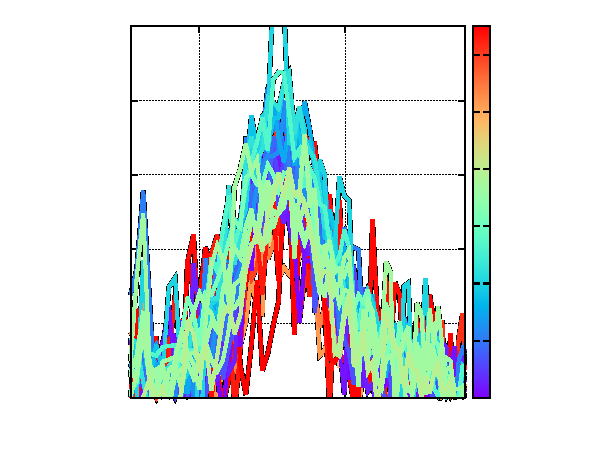
\includegraphics{CaelyxSucroseContinuousWAXS}}%
    \gplfronttext
  \end{picture}%
\endgroup
}\label{fig:CaelyxSucroseContinuousWAXS}}
		\subfloat[Diffraction peak width and position]{\resizebox{0.44\linewidth}{!}{% GNUPLOT: LaTeX picture with Postscript
\begingroup
  \makeatletter
  \providecommand\color[2][]{%
    \GenericError{(gnuplot) \space\space\space\@spaces}{%
      Package color not loaded in conjunction with
      terminal option `colourtext'%
    }{See the gnuplot documentation for explanation.%
    }{Either use 'blacktext' in gnuplot or load the package
      color.sty in LaTeX.}%
    \renewcommand\color[2][]{}%
  }%
  \providecommand\includegraphics[2][]{%
    \GenericError{(gnuplot) \space\space\space\@spaces}{%
      Package graphicx or graphics not loaded%
    }{See the gnuplot documentation for explanation.%
    }{The gnuplot epslatex terminal needs graphicx.sty or graphics.sty.}%
    \renewcommand\includegraphics[2][]{}%
  }%
  \providecommand\rotatebox[2]{#2}%
  \@ifundefined{ifGPcolor}{%
    \newif\ifGPcolor
    \GPcolortrue
  }{}%
  \@ifundefined{ifGPblacktext}{%
    \newif\ifGPblacktext
    \GPblacktextfalse
  }{}%
  % define a \g@addto@macro without @ in the name:
  \let\gplgaddtomacro\g@addto@macro
  % define empty templates for all commands taking text:
  \gdef\gplbacktext{}%
  \gdef\gplfronttext{}%
  \makeatother
  \ifGPblacktext
    % no textcolor at all
    \def\colorrgb#1{}%
    \def\colorgray#1{}%
  \else
    % gray or color?
    \ifGPcolor
      \def\colorrgb#1{\color[rgb]{#1}}%
      \def\colorgray#1{\color[gray]{#1}}%
      \expandafter\def\csname LTw\endcsname{\color{white}}%
      \expandafter\def\csname LTb\endcsname{\color{black}}%
      \expandafter\def\csname LTa\endcsname{\color{black}}%
      \expandafter\def\csname LT0\endcsname{\color[rgb]{1,0,0}}%
      \expandafter\def\csname LT1\endcsname{\color[rgb]{0,1,0}}%
      \expandafter\def\csname LT2\endcsname{\color[rgb]{0,0,1}}%
      \expandafter\def\csname LT3\endcsname{\color[rgb]{1,0,1}}%
      \expandafter\def\csname LT4\endcsname{\color[rgb]{0,1,1}}%
      \expandafter\def\csname LT5\endcsname{\color[rgb]{1,1,0}}%
      \expandafter\def\csname LT6\endcsname{\color[rgb]{0,0,0}}%
      \expandafter\def\csname LT7\endcsname{\color[rgb]{1,0.3,0}}%
      \expandafter\def\csname LT8\endcsname{\color[rgb]{0.5,0.5,0.5}}%
    \else
      % gray
      \def\colorrgb#1{\color{black}}%
      \def\colorgray#1{\color[gray]{#1}}%
      \expandafter\def\csname LTw\endcsname{\color{white}}%
      \expandafter\def\csname LTb\endcsname{\color{black}}%
      \expandafter\def\csname LTa\endcsname{\color{black}}%
      \expandafter\def\csname LT0\endcsname{\color{black}}%
      \expandafter\def\csname LT1\endcsname{\color{black}}%
      \expandafter\def\csname LT2\endcsname{\color{black}}%
      \expandafter\def\csname LT3\endcsname{\color{black}}%
      \expandafter\def\csname LT4\endcsname{\color{black}}%
      \expandafter\def\csname LT5\endcsname{\color{black}}%
      \expandafter\def\csname LT6\endcsname{\color{black}}%
      \expandafter\def\csname LT7\endcsname{\color{black}}%
      \expandafter\def\csname LT8\endcsname{\color{black}}%
    \fi
  \fi
  \setlength{\unitlength}{0.0500bp}%
  \begin{picture}(5668.00,4534.00)%
    \gplgaddtomacro\gplbacktext{%
      \csname LTb\endcsname%
      \put(814,1028){\makebox(0,0)[r]{\strut{}-1}}%
      \csname LTb\endcsname%
      \put(814,1838){\makebox(0,0)[r]{\strut{}-0.5}}%
      \csname LTb\endcsname%
      \put(814,2649){\makebox(0,0)[r]{\strut{} 0}}%
      \csname LTb\endcsname%
      \put(814,3459){\makebox(0,0)[r]{\strut{} 0.5}}%
      \csname LTb\endcsname%
      \put(814,4269){\makebox(0,0)[r]{\strut{} 1}}%
      \csname LTb\endcsname%
      \put(1084,484){\makebox(0,0){\strut{} 250}}%
      \csname LTb\endcsname%
      \put(1922,484){\makebox(0,0){\strut{} 500}}%
      \csname LTb\endcsname%
      \put(2759,484){\makebox(0,0){\strut{} 750}}%
      \csname LTb\endcsname%
      \put(3596,484){\makebox(0,0){\strut{} 1000}}%
      \csname LTb\endcsname%
      \put(4434,484){\makebox(0,0){\strut{} 1250}}%
      \csname LTb\endcsname%
      \put(5271,484){\makebox(0,0){\strut{} 1500}}%
      \put(176,2486){\rotatebox{-270}{\makebox(0,0){\strut{}Diffraction Peak Deviation / $\%$}}}%
      \put(3108,154){\makebox(0,0){\strut{}Solvent Osmolality / mOsm kg$^{-1}$}}%
    }%
    \gplgaddtomacro\gplfronttext{%
    }%
    \gplbacktext
    \put(0,0){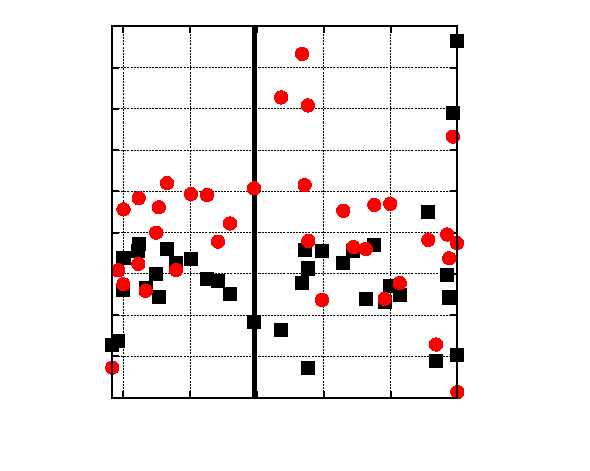
\includegraphics{CaelyxSucroseContinuousWAXSDiffraction}}%
    \gplfronttext
  \end{picture}%
\endgroup
}\label{fig:CaelyxSucroseContinuousWAXSDiffraction}}
		\caption{Measured in WAXS, the $q$-region where the doxorubicin diffraction peak appears can be observed. With black symbols, the shift of the doxorubicin-aggregate diffraction peak from $q=0.123$ nm$^{-1}$ is displayed The mean width (FWHM) is 0.333  nm$^{-1}$}
\end{figure}

To conclude this section, the diameter obtained from the isoscattering position in the aqueous iodixanol solution can be compared with what is measured in an aqueous sucrose suspending medium.  In the latter, if only the scattering curves below this osmolality threshold are considered, the relative standard deviation for each q value reveals a pronounced minimum for the first isoscattering point as depicted in Fig. 6. When comparing this result with the relative standard deviation curve obtained from the Optiprep TM contrast variation measurements, both values for the size of the drug carrier agree remarkably well within 0.8 $\%$. This reflects the independence of the technique from the contrast agent added to the suspending medium and shows the repeatability of the results.

\begin{figure}
	\centering
		% GNUPLOT: LaTeX picture with Postscript
\begingroup
  \makeatletter
  \providecommand\color[2][]{%
    \GenericError{(gnuplot) \space\space\space\@spaces}{%
      Package color not loaded in conjunction with
      terminal option `colourtext'%
    }{See the gnuplot documentation for explanation.%
    }{Either use 'blacktext' in gnuplot or load the package
      color.sty in LaTeX.}%
    \renewcommand\color[2][]{}%
  }%
  \providecommand\includegraphics[2][]{%
    \GenericError{(gnuplot) \space\space\space\@spaces}{%
      Package graphicx or graphics not loaded%
    }{See the gnuplot documentation for explanation.%
    }{The gnuplot epslatex terminal needs graphicx.sty or graphics.sty.}%
    \renewcommand\includegraphics[2][]{}%
  }%
  \providecommand\rotatebox[2]{#2}%
  \@ifundefined{ifGPcolor}{%
    \newif\ifGPcolor
    \GPcolortrue
  }{}%
  \@ifundefined{ifGPblacktext}{%
    \newif\ifGPblacktext
    \GPblacktextfalse
  }{}%
  % define a \g@addto@macro without @ in the name:
  \let\gplgaddtomacro\g@addto@macro
  % define empty templates for all commands taking text:
  \gdef\gplbacktext{}%
  \gdef\gplfronttext{}%
  \makeatother
  \ifGPblacktext
    % no textcolor at all
    \def\colorrgb#1{}%
    \def\colorgray#1{}%
  \else
    % gray or color?
    \ifGPcolor
      \def\colorrgb#1{\color[rgb]{#1}}%
      \def\colorgray#1{\color[gray]{#1}}%
      \expandafter\def\csname LTw\endcsname{\color{white}}%
      \expandafter\def\csname LTb\endcsname{\color{black}}%
      \expandafter\def\csname LTa\endcsname{\color{black}}%
      \expandafter\def\csname LT0\endcsname{\color[rgb]{1,0,0}}%
      \expandafter\def\csname LT1\endcsname{\color[rgb]{0,1,0}}%
      \expandafter\def\csname LT2\endcsname{\color[rgb]{0,0,1}}%
      \expandafter\def\csname LT3\endcsname{\color[rgb]{1,0,1}}%
      \expandafter\def\csname LT4\endcsname{\color[rgb]{0,1,1}}%
      \expandafter\def\csname LT5\endcsname{\color[rgb]{1,1,0}}%
      \expandafter\def\csname LT6\endcsname{\color[rgb]{0,0,0}}%
      \expandafter\def\csname LT7\endcsname{\color[rgb]{1,0.3,0}}%
      \expandafter\def\csname LT8\endcsname{\color[rgb]{0.5,0.5,0.5}}%
    \else
      % gray
      \def\colorrgb#1{\color{black}}%
      \def\colorgray#1{\color[gray]{#1}}%
      \expandafter\def\csname LTw\endcsname{\color{white}}%
      \expandafter\def\csname LTb\endcsname{\color{black}}%
      \expandafter\def\csname LTa\endcsname{\color{black}}%
      \expandafter\def\csname LT0\endcsname{\color{black}}%
      \expandafter\def\csname LT1\endcsname{\color{black}}%
      \expandafter\def\csname LT2\endcsname{\color{black}}%
      \expandafter\def\csname LT3\endcsname{\color{black}}%
      \expandafter\def\csname LT4\endcsname{\color{black}}%
      \expandafter\def\csname LT5\endcsname{\color{black}}%
      \expandafter\def\csname LT6\endcsname{\color{black}}%
      \expandafter\def\csname LT7\endcsname{\color{black}}%
      \expandafter\def\csname LT8\endcsname{\color{black}}%
    \fi
  \fi
  \setlength{\unitlength}{0.0500bp}%
  \begin{picture}(5668.00,4534.00)%
    \gplgaddtomacro\gplbacktext{%
      \csname LTb\endcsname%
      \put(946,638){\makebox(0,0)[r]{\strut{} 0}}%
      \csname LTb\endcsname%
      \put(946,1243){\makebox(0,0)[r]{\strut{} 0.05}}%
      \csname LTb\endcsname%
      \put(946,1848){\makebox(0,0)[r]{\strut{} 0.1}}%
      \csname LTb\endcsname%
      \put(946,2454){\makebox(0,0)[r]{\strut{} 0.15}}%
      \csname LTb\endcsname%
      \put(946,3059){\makebox(0,0)[r]{\strut{} 0.2}}%
      \csname LTb\endcsname%
      \put(946,3664){\makebox(0,0)[r]{\strut{} 0.25}}%
      \csname LTb\endcsname%
      \put(946,4269){\makebox(0,0)[r]{\strut{} 0.3}}%
      \csname LTb\endcsname%
      \put(1194,418){\makebox(0,0){\strut{} 0.1}}%
      \csname LTb\endcsname%
      \put(2359,418){\makebox(0,0){\strut{} 0.15}}%
      \csname LTb\endcsname%
      \put(3524,418){\makebox(0,0){\strut{} 0.2}}%
      \csname LTb\endcsname%
      \put(4689,418){\makebox(0,0){\strut{} 0.25}}%
      \put(176,2453){\rotatebox{-270}{\makebox(0,0){\strut{}Relative Standard Deviation}}}%
      \put(3174,154){\makebox(0,0){\strut{}$q$ / nm$^{-1}$}}%
    }%
    \gplgaddtomacro\gplfronttext{%
      \csname LTb\endcsname%
      \put(4548,4041){\makebox(0,0)[r]{\strut{}\smaller Optiprep}}%
      \csname LTb\endcsname%
      \put(4548,3711){\makebox(0,0)[r]{\strut{}\smaller Aqueous sucrose}}%
    }%
    \gplbacktext
    \put(0,0){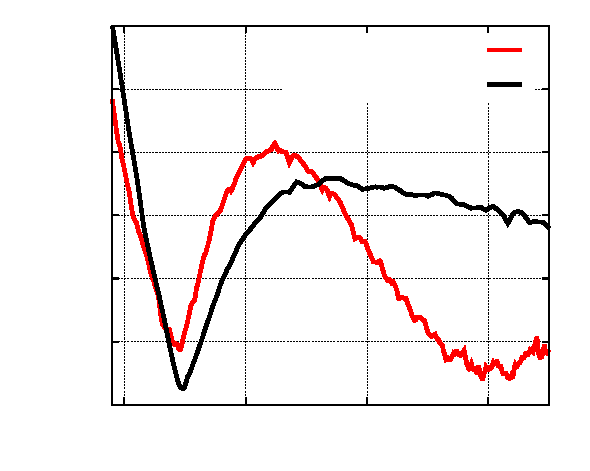
\includegraphics{CaelyxIsopointComparison}}%
    \gplfronttext
  \end{picture}%
\endgroup

		\caption{Isoscattering point position quantified by the calculation of the relative standard deviation of the scattering curves for different solvent density gradients. In the case of the aqueous sucrose solution (black line), only the scattering curves below the osmolality threshold were employed for the calculation.}
		\label{fig:CaelyxIsopointComparison}
\end{figure}

\subsection{Size dependency of the osmotic activity}

\section{Application to blood plasma componenents}
\subsection{HDL}
\subsection{LDL}
\subsection{Literature comparison}

\section{Protein-coated low-density nanoparticles}
\subsection{Singe-contrast SAXS}
Caterina Minelli Paper ECASIA
\subsection{Contrast variation}
Isopoint subtraction, as in BioSurf

\section{Summary}
This article demonstrates that it is possible to determine the size of a PEGylated liposomal drug carrier with continuous contrast variation in SAXS. By means of an iso-osmolal density gradient, the position of the isoscattering point was measured whereby the size of the liposomal drug was determined. Supplemented by the model fitting of the so called shape factor of the liposomes, the size was also obtained from an independent evaluation procedure and an average size of (69 $\pm$ 5) nm was obtained. This size is smaller than the value measured by DLS, which can be attributed to the fact that the contrast variation SAXS determines the size of the liposomes impermeable to the contrast agent, i.e. the outer PEG layer of the liposomes is not probed. The latter implies that the combination of SAXS with DLS can reveal the difference between the hydrodynamic diameter and the "core" size of the nanocarrier, which is related to the thickness of the PEG-layer in case of stealth liposomes. Moreover the method presented in this paper shows that by means of the shape factor fitting, complementary information about the shape of the nanocarrier can be obtained.

Using an aqueous sucrose density gradient, it was shown that an increasing osmolality of the buffer produces an osmotic shrinkage of the liposomal structure, although this structural deformation is reversible and does not affect the crystalline structure of the intraliposomal doxorubicin.

These results, together with the determination of the average electron density of the liposomal doxorubicin of (346.2 $\pm$ 1.2) nm$^{-3}$, demonstrate the applicability of the density gradient technique for complex particles. This model-free approach to contrast variation in SAXS proves to be a powerful sizing technique, which, in addition, makes it possible to study simultaneously the behavior of the liposomal drug carrier under different osmotic conditions.

